\section{Material und Methoden}
%
%CALIBRIERUNG:
%LAsUFBAND 		   :	    245 pix = 1 m 
%LAUFSTRECKE		: 		260 pix = 1 m
%

\subsection{Proband}
Die Untersuchungen wurden an einer männlichen Person, 24 Jahre, 1,86\,m Körpergröße, 83\,kg Körpergewicht durchgeführt. Zum leichteren verfolgen der Gelenke wurden neun reflektierende Marker auf der linken Körperseite auf Ferse, Fußballen, Knöchel, Knie, Hüfte, Schulter, Hals, Ellenbogen und Handgelenk aufgebracht. Alle Laufversuche wurden ohne Schuhwerk, aber mit Socken durchgeführt.

\subsection{Laufband}
Die Laufbandversuche wurden durchgeführt auf einem mercury 4.0 Laufband (h/p/cosmos sports \& medical GmbH, Nussdorf-Traunstein, Deutschland). Videos wurden mit einer Samsung VP-HMX20C Videokamera (Samsung AG Seoul, Südkorea) mit einer Bildrate von 50~Hz, einer Belichtung von 1/1000~s und auf 5~m fixierten Fokus aufgenommen. 
Zur Ausleuchtung wurden zwei weißen 500W Baustrahlern aufgestellt. Abbildung~\ref{fig:laufbnd_stp} zeigt den Aufbau.\\
\begin{wrapfigure}{r}{6.5cm}
	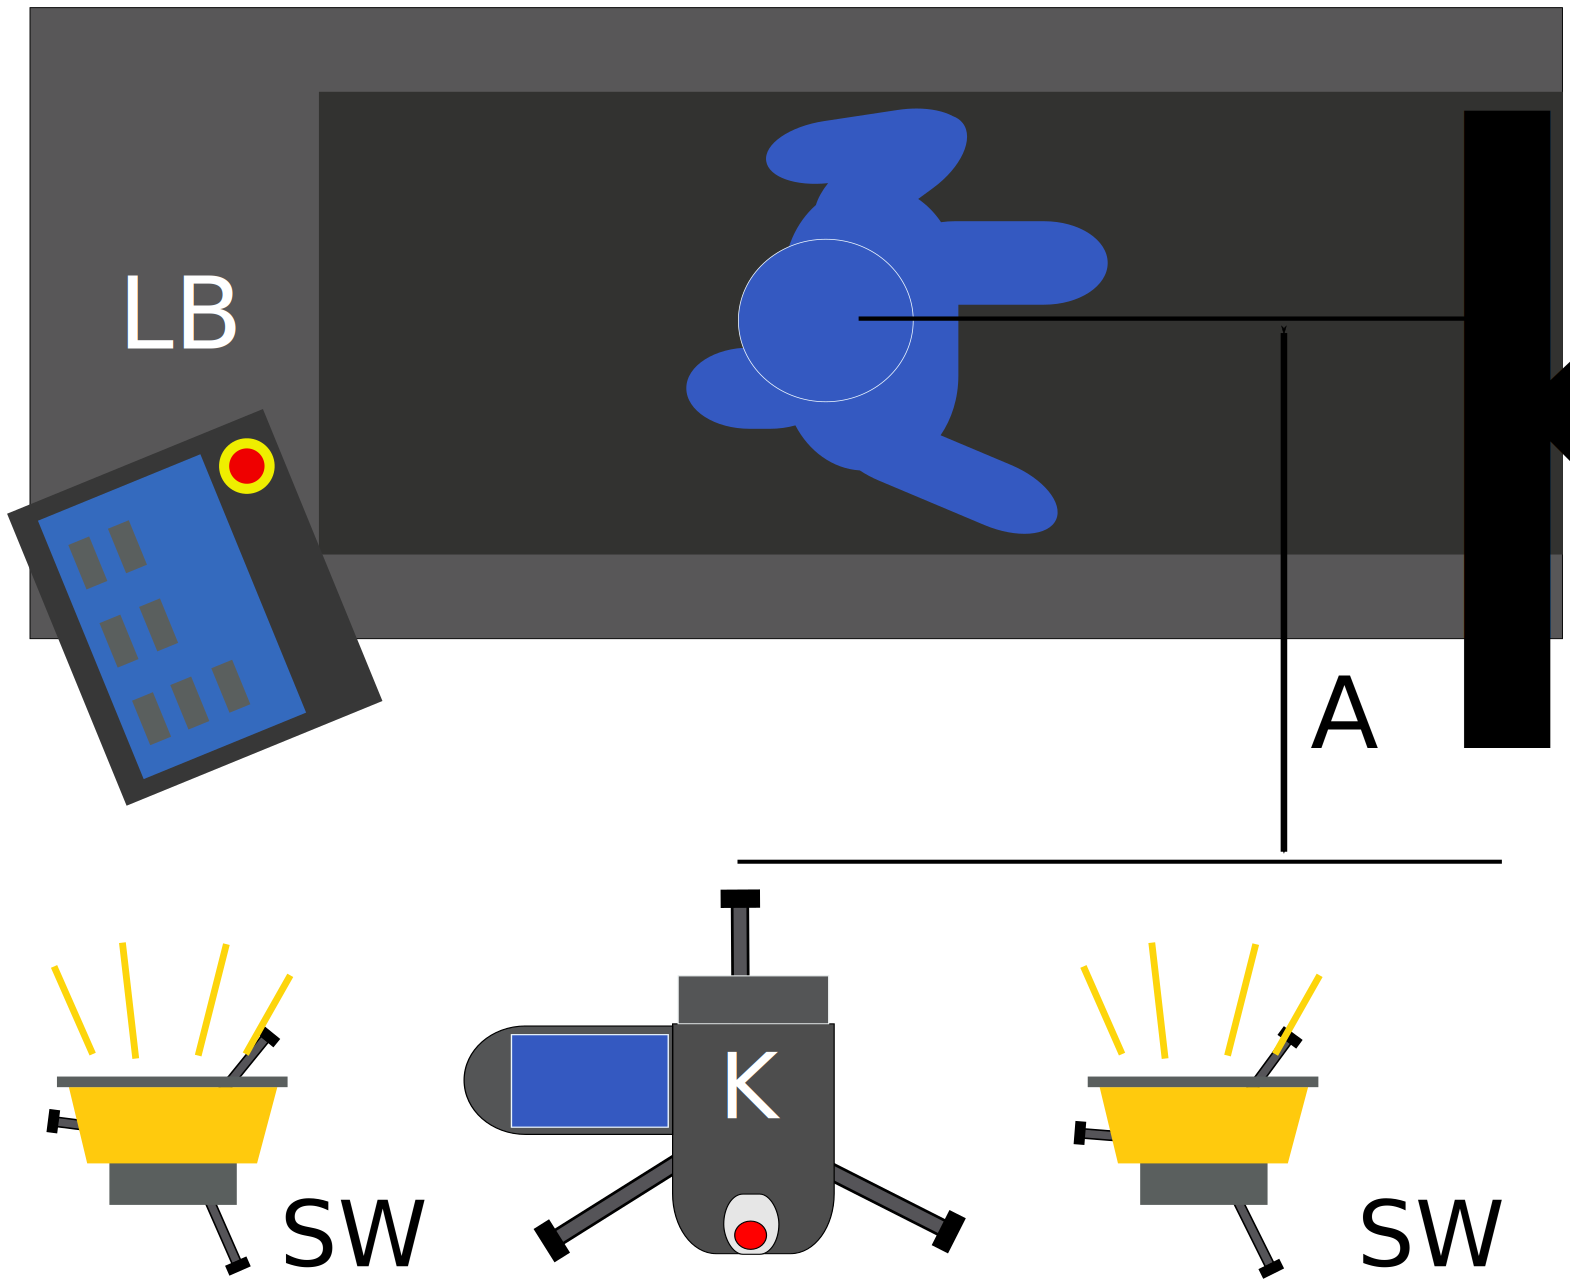
\includegraphics[width=\linewidth]{bilder/mat_met/Laufband_setup}
	\caption[Aufbau Laufband Versuch]{Aufbau des Laufband-Versuches mit Laufband LB, Kamera K und Scheinwerfern SW. Abstand zur Kamera $A_{Kam}$~=~5~m }
	\label{fig:laufbnd_stp}
\end{wrapfigure}

Es sollen sieben Gehgeschwindigkeiten untersucht werden. Hierfür wurden pro Geschwindigkeit jeweils mehrere Gangzyklen aufgenommen.\\
Bevor 
Nachdem sich der Proband an das Laufen auf dem Laufband gewöhnt hat, werden die Geschwindigkeiten von 1 bis 7\,km/h in 1\,km/h Schritten untersucht. Vor jeder neuen Videoaufnahme wird die Geschwindigkeit erhöht und der Proband hat Zeit, sich an die Geschwindigkeit anzupassen. Dabei wird auch eine subjektive Einschätzung verlangt, als wie anstrengend oder angenehm die aktuelle Laufgeschwindigkeit empfunden wird. Die subjektiven Einschätzungen werden nach Abschluss der Versuche in Werte von 1 (sehr unangenehm) bis 10 (sehr angenehm) überführt.\\

\subsection{Laufstrecke mit Kraftmessplatte}
Für die Versuche auf der Laufstrecke soll der Proband in drei Geschwindigkeiten, welche als {langsam}, angenehm und schnell eingeschätzt werden, über die Laufstrecke gehen und dabei auf der Waage mit seinem linken Fuß möglichst zentral auftreten.\\
Videokamera und Baustrahler des Laufband-Versuches kommen auch hier zum Einsatz. Die Laufstrecke ist ein Eigenbau der Hochschule Bremen. Ein Quarzkristall-3-Komponenten-Dynanometer Typ 9257B (Kistler Gruppe Winterthur, Schweiz), im Folgenden {Waage} genannt, wird unter einer Platte (\textbf{ABMESSUNGEN}) eingebaut. Die Waage ist über einen Mehrkanal-Ladungsverstärker Typ 5070A (Kistler) mit einem Computer verbunden. Abbildung~\ref{fig:laufstg_stp} zeigt den Aufbau. Die Kamera steht zentriert vor der Waage und die Bildebene ist parallel zur Saggitalebene ausgerichtet.
Das Waagenzentrum liegt in den Aufnahmen bei x = 1.554\,m, y = 0.099\,m von der linken unteren Bildecke aus.
\begin{figure}[h!]
	\centering
	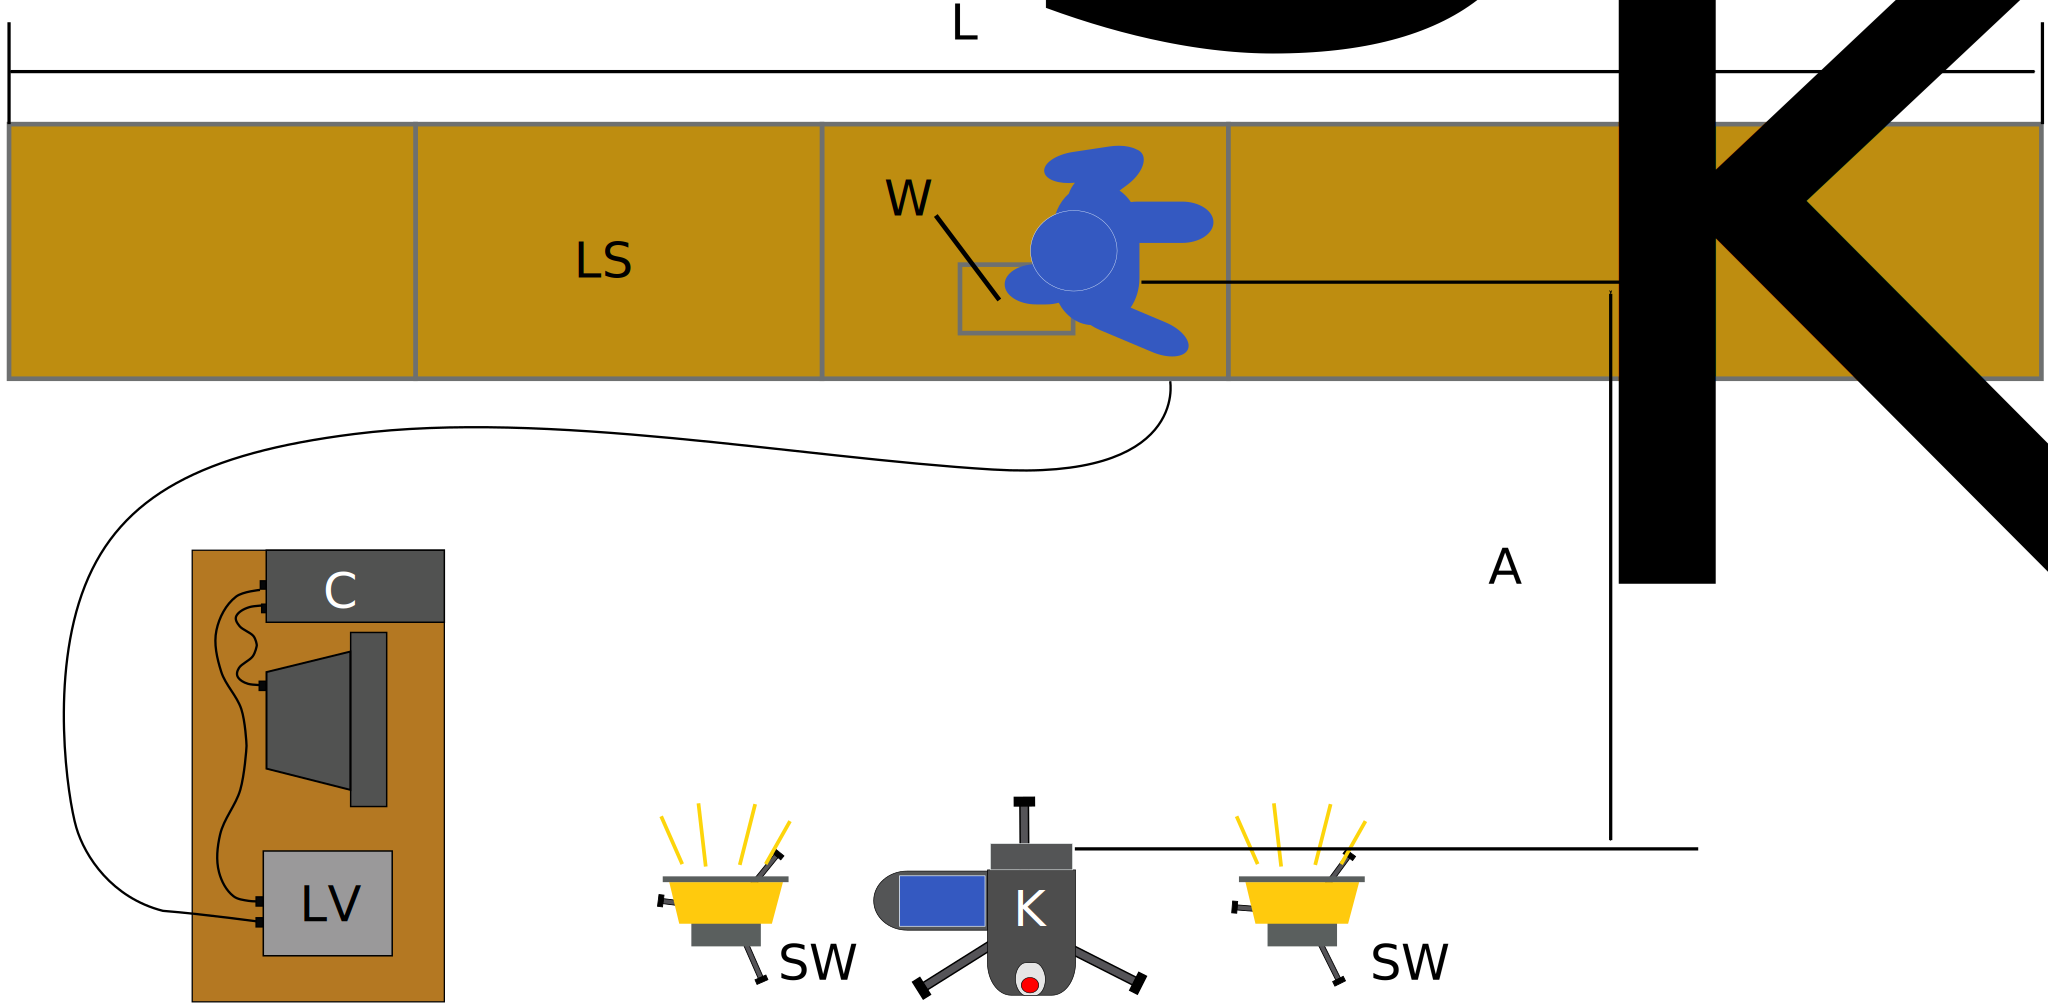
\includegraphics[width=0.7\linewidth]{bilder/mat_met/Laufstrecke_setup}
	\caption[Aufbau Laufstrecke Versuch]{Aufbau des Laufstrecke-Versuches mit Laufstrecke LS, Kamera K, Scheinwerfern SW, Computer C, Waage W und Ladungsverstärker LV. Länge Steg $L_S~=~6~m$ und Abstand zur Kamera $A_{Kam}~=~5~m$}
	\label{fig:laufstg_stp}
\end{figure}

Die Kameraeinstellungen vom Laufbandversuch übernommen finden auch hier Anwendung. Die Digitalisierung der Koordinaten ist wie oben beschrieben durchgeführt worden. Die Waagensignale werden mit 100\,Hz und 200\,N/V vom Ladungsverstärker an den Computer weitergeleitet. Mit DASYLab (Measurement Computing, Norton, USA) werden die Eingangssignale verarbeitet und alle 8 Kanäle im ASCII-Format gespeichert.
Für eine 4-Punkt-Kalibration wird die Waage in alle drei Raumrichtungen mit 0, 1, 3,6 und 7,75\,kg belastet. Der Waagendrift wird über 30\,s ohne Belastung für jede Raumrichtung ermittelt.\\
Das Gehen über die Waage muss einige Male geübt werden, so dass die Waage mit dem Linken Fuß möglichst zentral belastet wird, dies aber nicht durch eine Änderung des Ganges erreicht wird. 

\subsection{Datenauswertung}
Alle verwendeten Videos werden mit dem Programm ffmpeg 2.1 (LGP License, ffmpeg.org) in Einzelbilder zerlegt. Es wird für jeden Versuch eine Bildsequenz ausgewählt, welche einem Schritt (linkes Bein abheben, schwingen, aufsetzen, belasten und entlasten) entspricht. Das Programm ImageJ (National Institutes of Health Bethesda, Maryland) mit dem Plugins MTrackJ \textbf{CITE(Meijering 20120)} erlaubt dann das Erfassen der xy-Koordinaten der Gelenke in jedem Einzelbild. Für die sieben ausgewählten Bildsequenzen des Laufbandexperiments und die drei Sequenzen des Laufstreckenexperiments werden jeweils neun Marker verfolgt und der Datensatz im .mdf-Format gespeichert.
Die Dauer der Schwungphase, der Standphase und des gesamten Schrittzyklus sowie der Duty-Faktor werden aus den Bildsequenzen bestimmt. Der Dutyfaktor ist wie folgt definiert:
\begin{equation}
\mathrm{DF} = \frac{\mathrm{T_{Stand}}}{\mathrm{T_{Schritt}}}
\end{equation}
Die weitere Auswertung der erhaltenen Trajektorien und Waagenausgabe erfolgt in der Skriptsprache Scilab (Scilab Enterprises S.A.S., Orsay Cedex, France). Im folgenden sollen die verwendeten Algorithmen beschrieben werden, für die  genaue Implementierung sei auf den Quellquode auf der beigefügte CD.\\
\subsubsection{Datenstruktur}
In einem objektorientierten Ansatz werden Strukturen geschaffen, welche ein möglichst gut verständliches Abbild der physikalisch-biologischen Beschreibung bieten. Dies wird erreicht durch eine Schachelung von Containern und Eigenschaften. Der Datensatz eines Experiments wird so zusammengefasst in einem 'Körper', der Körper beinhaltet nun alle Gelenke und Körpersegmente, welche wiederum ihre Eigenschaften wie Masse und Trägheitsradius, sowie den zeitlichen Verlauf von Ort, Geschwindigkeit, Winkel etc. beinhalten. 
\subsubsection{Numerische Verfahren}
Die Geschwindigkeit eines Punktes ergibt sich aus der zeitlichen Ableitung seines Ortes. Die Bestimmung der Geschwindigkeit v zum Zeitpunkt t aus diskreten Ortswerten $\mathrm{x(t - \Delta{t})}$ und $\mathrm{x(t + \Delta{t})}$wird durch die Verwendung der Zentraldifferenz durchgeführt:
\begin{equation}
	\vec{v}(t) = \frac{\vec{x}(t + \Delta{t}) - \vec{x}(t - \Delta{t})}{2\Delta{t}}
\end{equation}
Für die Randwerte, d.h. den ersten und letzten Mittelwert, wird mangels Stützstellen eine Vorwärts-, beziehungsweise Rückwärtsdifferenz durchgeführt.
Abgeleitete Daten wie Geschwindigkeit, Beschleunigung und Winkel, sowie die Kraftwerte werden durch einen gleitenden Mittelwert geglättet:
\begin{equation}
	    \vec{\phi}(t) = \frac{a\,\phi(t - \Delta{t}) + b\,\phi(t) + c\,\phi(t - \Delta{t})}{a + b + c}
\end{equation}
Werden die Gewichtungsfaktoren a, b und c auf 1 gesetzt, erhält man einen gleitenden Mittelwert mit drei Stützstellen. Ein Ändern der Gewichtungsfaktoren erzeugt einen gewichteten Mittelwert. Die Randwerte werden hierbei nicht geglättet.\\
Der Winkel zwischen zwei Gelenken wird durch triviale Trigonometrie berechnet und ist in den Ergebnissen, falls keine weitere Erläuterung vorhanden ist, jeweils im mathematischen Sinne und in Grad angegeben. 

\subsubsection{Anthropometrie}
Mit Hilfe der Tabelle \textbf{NEED TABELLE} können die Eigenschaften eines Segmentes aus dem Körpergewicht, sowie den Ortsvektoren von den benachbarten Gelenken bestimmt werden. CoM (center of mass) steht für den Masseschwerpunkt, d für das distale Gelenk und p für das proximale Gelenk. Der Ortsvektor des Masseschwerpunktes eines Segmentes wird mit Hilfe eines Faktors $c_{seg}$ aus der Antropometrietabelle berechnet:
\begin{equation}
\vec{x}_{CoM} = (\vec{x}_d - \vec{x}_p) \cdot c_{seg} + \vec{x}_p
\label{eq:CoM_x}
\end{equation}

\subsection{Auswertung Laufband}
Die Frequenz des Beinschwingens wird mit der Frequenz eines mathematischen Pendels verglichen. Die Frequenz des Schwingens ergibt sich aus der Zeit zwischen Abheben und Aufsetzen eines Fußes. Die Frequenz ist der Kehrwert der Periodendauer, eine Periode bezeichnet das Hin- und Zurückschwingen des Pendels, weshalb $\mathrm{T_{Schwung}}$ mit zwei multipliziert wird:
\begin{equation}
\mathrm{f_{Schwung}} = 1 / (2 * (\mathrm{T_{Schwung}}))
\end{equation}
Die Periodendauer T eines mathematischen Pendels (konstante Länge L zwischen Aufhängung und Punktmasse) ergibt sich aus:
\begin{equation}
	T = 2  \pi \sqrt{\frac{L}{g}} 
\end{equation}
Diese Gleichung gilt für kleine Auslenkungswinkel ($\le$ 5 Grad). Die Pendellänge L wird bestimmt als der Abstand zwischen der Aufhängung Hüfte und des Masseschwerpunktes des gesamten Beines.
Als Vergleich und Validierung wird die eingestellte Laufbandgeschwindigkeit zwei Berechnungsmethoden gegenübergestellt. Die Geschwindigkeit lässt sich aus den Videodateien als diejenige definieren, mit der sich der Fuß fortbewegt, wenn er fest auf dem Band steht. Weiterhin kann die Fortbewegungsgeschwindigkeit des Probanden relativ zum Laufband aus der doppelten Schrittfrequenz und der Schrittweite pro Schritt bestimmt werden.
\begin{equation}
v_{\mathrm{calc}} = f_{\mathrm{fSchritt}} \cdot 2 \cdot x_{\mathrm{Schritt}} \cdot 3,6\;\frac{\mathrm{km/h}}{\mathrm{m/s}}
\end{equation}

\subsubsection{Inverse Dynamik}
Die inverse Dynamik erlaubt die Bestimmung von Kraft und Momenten in Gelenken, ohne Messungen an den jeweiligen Gelenken durchführen zu müssen. Hierfür werden die Segmente zwischen zwei Gelenken als Balkenelemente abstrahiert und die Gelenke als einfache Lager. Durch Aufstellen von Kraft- und Momentengleichgewichten können, ausgehend von der auf die Waage wirkenden Kräfte in Knöchel, Knie und Hüfte bestimmt werden. Die aufgestellten Gleichungen sind im Anhang zu finden.

\subsubsection{Vergleich Laufband - Laufstrecke}
Die Neigung des Oberkörpers wird durch den Winkel, welcher zwischen der Verbindung von Hüfte zu Nacken und der x Koordinate anliegt. Ein Winkel von 0 Grad entspricht dabei einem aufrechten Oberkörper, postive Winkel einer Vorbeugung, negative Winkel zeigen einen nach hinten gebeugten Oberkörper an. \\
Um die Trajektorien der Hände vergleichbar machen zu können, wird der Ortsvektor des Handgelenks relativ zum Nacken dargestellt. 






